\documentclass[12pt]{article}

\usepackage{graphicx}
\usepackage{biblatex} %Imports biblatex package
\usepackage{subfig}
\usepackage{caption}
\usepackage{hyperref}
\usepackage{amsmath}
\addbibresource{./report.bib} %Import the bibliography file


%set title
\title{Challenge 1}
\author{Francesco Ortu}




\begin{document}
\maketitle
\begin{abstract}

\end{abstract}

\section{Introduction}
 The aim of the Challenge 1 is to investigate the FashionMNIST \cite{xiao2017/online} dataset.
 The task was to create a pipeline using Kernel methods and ANNs, using both unsupervised and supervised methods.
 The code is available ..
 \section{Dataset}
 The dataset used contains 70,000 images of 10 different classes. The images are 28x28 grayscale images. The dataset is divided in 60,000 training images and 10,000 test images. The classes are: T-shirt/top, Trouser, Pullover, Dress, Coat, Sandal, Shirt, Sneaker, Bag, Ankle boot.
 I imported the dataset using the torchvision package. However, I selected randomically the $40000$ images from the $60000$ of the train test, due to computational cost.

 \section{Exploring geometry of the data}
The first question addressed was to investigate the geometry of the data. To do so, I perform
a PCA and kernel PCA with $3$ principal components. The hyperparameters were choosen in order to obtain the best results possible by visual inspection.
The results are shown in the Figure \ref{fig:pca}. In the associated 
notebook there is also a interactive 3D plot, that could be useful to understand better the geometry of the transformed data.


\begin{figure}[htbp]
    \centering
    {\subfloat[linear]{\includegraphics[width=0.45\textwidth]{./images/linear_PCA.png}}}\hfill
    {\subfloat[Gaussian kernel]{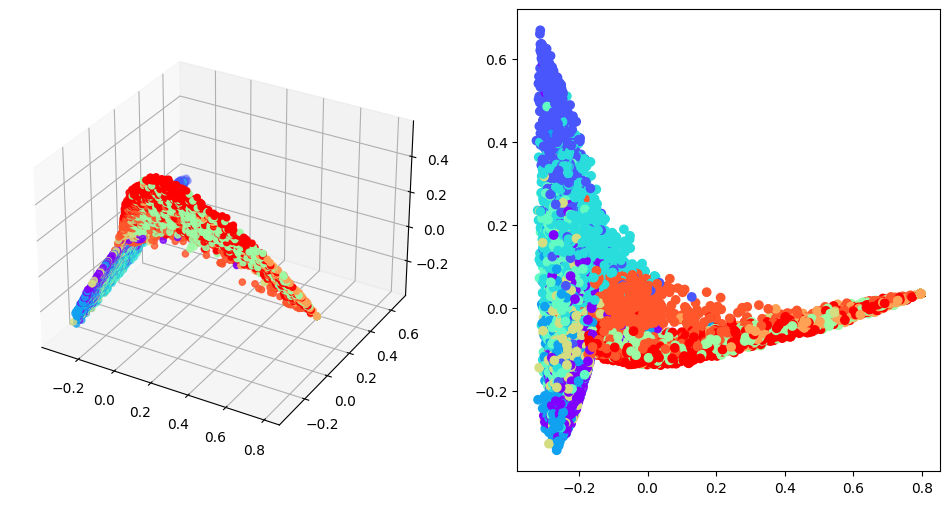
\includegraphics[width=0.45\textwidth]{./images/rfb_pca.png}}}\\
    {\subfloat[Polynomial kernel]{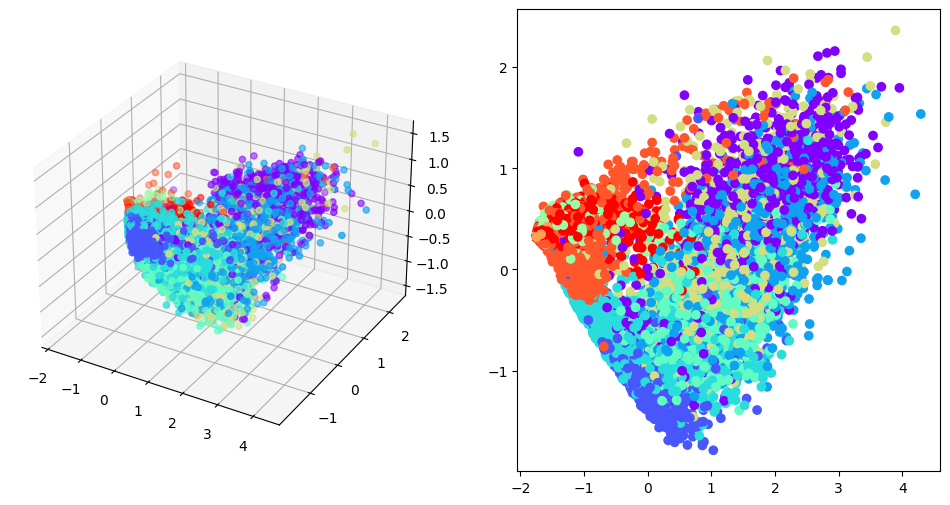
\includegraphics[width=0.45\textwidth]{./images/polinomial_pca.png}}}\hfill
    {\subfloat[Cosine]{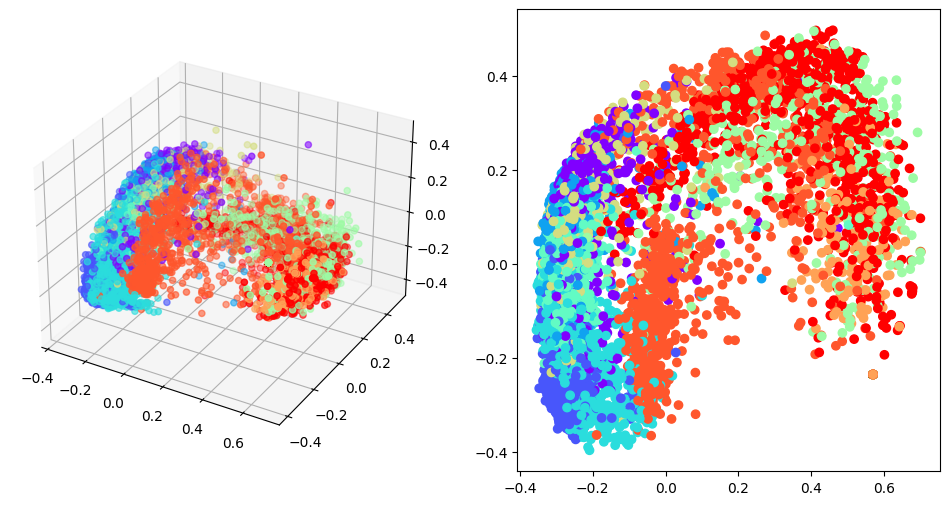
\includegraphics[width=0.45\textwidth]{./images/cosine_pca.png}}}
    \caption{Pca and kernel PCA }
    \label{fig:pca}
    
\end{figure}

From the results, it is possible to see that the data are not easly separable. It is seems that the dara are more separable with the Linear PCA then with the other kernel. 
However, with a better intuiton about the geometry of the data, could be constructed a kernel that could perform better.

\section{Unsupervised labelling of the data}
I choose the linear PCA to label the data, using k-means to clustering. I have also tried the Expectation-Maximization algorithm, because it seems from the previous section
that the data points of different label follow a gaussian distribution. However, the performance obtained with kmeans are comparable with the EM algorithm, but with a less computational cost.
In order to compare the performance, I mapped the label obtained with the clustering algorithm to the true label, assigned to each cluster the most frequent real label of his data point.
Doing so, however, two cluster are mapped to the same one. I decided to not force the procedure in order to have a 1-1 map, because I believe that the problem are in the way the data are trasformed using PCA.
Probably, with a better kernel the cluster will not be clusters that overlap with others. The accuracy obtained is about $60\%$, and the results are shown in Figure \ref{fig:map_pca}.

\begin{figure}[htbp]
    \centering
    {\subfloat[2D]{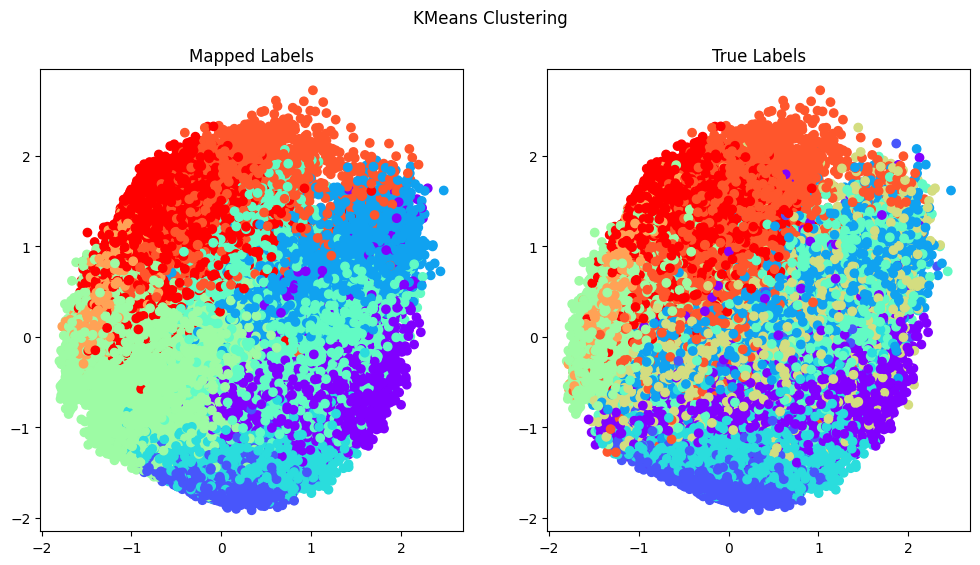
\includegraphics[width=0.6\textwidth]{./images/map_pca.png}}}\\
    {\subfloat[3D]{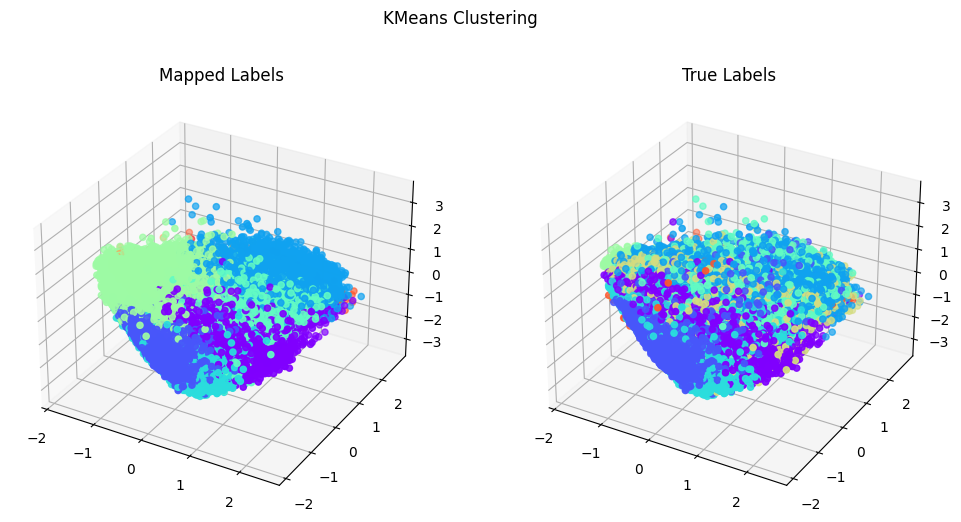
\includegraphics[width=0.6\textwidth]{./images/map_pca3D.png}}}

    \caption{Unsupervised mapped label against the true ones}
    \label{fig:map_pca}
    
\end{figure}
 

%

\end{document}